\documentclass[]{book}
\usepackage{lmodern}
\usepackage{amssymb,amsmath}
\usepackage{ifxetex,ifluatex}
\usepackage{fixltx2e} % provides \textsubscript
\ifnum 0\ifxetex 1\fi\ifluatex 1\fi=0 % if pdftex
  \usepackage[T1]{fontenc}
  \usepackage[utf8]{inputenc}
\else % if luatex or xelatex
  \ifxetex
    \usepackage{mathspec}
  \else
    \usepackage{fontspec}
  \fi
  \defaultfontfeatures{Ligatures=TeX,Scale=MatchLowercase}
\fi
% use upquote if available, for straight quotes in verbatim environments
\IfFileExists{upquote.sty}{\usepackage{upquote}}{}
% use microtype if available
\IfFileExists{microtype.sty}{%
\usepackage{microtype}
\UseMicrotypeSet[protrusion]{basicmath} % disable protrusion for tt fonts
}{}
\usepackage[unicode=true]{hyperref}
\hypersetup{
            pdftitle={PSC 253 Minimal Manual},
            pdfauthor={Matthew B. Platt},
            pdfborder={0 0 0},
            breaklinks=true}
\urlstyle{same}  % don't use monospace font for urls
\usepackage{natbib}
\bibliographystyle{plainnat}
\usepackage{color}
\usepackage{fancyvrb}
\newcommand{\VerbBar}{|}
\newcommand{\VERB}{\Verb[commandchars=\\\{\}]}
\DefineVerbatimEnvironment{Highlighting}{Verbatim}{commandchars=\\\{\}}
% Add ',fontsize=\small' for more characters per line
\usepackage{framed}
\definecolor{shadecolor}{RGB}{248,248,248}
\newenvironment{Shaded}{\begin{snugshade}}{\end{snugshade}}
\newcommand{\KeywordTok}[1]{\textcolor[rgb]{0.13,0.29,0.53}{\textbf{{#1}}}}
\newcommand{\DataTypeTok}[1]{\textcolor[rgb]{0.13,0.29,0.53}{{#1}}}
\newcommand{\DecValTok}[1]{\textcolor[rgb]{0.00,0.00,0.81}{{#1}}}
\newcommand{\BaseNTok}[1]{\textcolor[rgb]{0.00,0.00,0.81}{{#1}}}
\newcommand{\FloatTok}[1]{\textcolor[rgb]{0.00,0.00,0.81}{{#1}}}
\newcommand{\ConstantTok}[1]{\textcolor[rgb]{0.00,0.00,0.00}{{#1}}}
\newcommand{\CharTok}[1]{\textcolor[rgb]{0.31,0.60,0.02}{{#1}}}
\newcommand{\SpecialCharTok}[1]{\textcolor[rgb]{0.00,0.00,0.00}{{#1}}}
\newcommand{\StringTok}[1]{\textcolor[rgb]{0.31,0.60,0.02}{{#1}}}
\newcommand{\VerbatimStringTok}[1]{\textcolor[rgb]{0.31,0.60,0.02}{{#1}}}
\newcommand{\SpecialStringTok}[1]{\textcolor[rgb]{0.31,0.60,0.02}{{#1}}}
\newcommand{\ImportTok}[1]{{#1}}
\newcommand{\CommentTok}[1]{\textcolor[rgb]{0.56,0.35,0.01}{\textit{{#1}}}}
\newcommand{\DocumentationTok}[1]{\textcolor[rgb]{0.56,0.35,0.01}{\textbf{\textit{{#1}}}}}
\newcommand{\AnnotationTok}[1]{\textcolor[rgb]{0.56,0.35,0.01}{\textbf{\textit{{#1}}}}}
\newcommand{\CommentVarTok}[1]{\textcolor[rgb]{0.56,0.35,0.01}{\textbf{\textit{{#1}}}}}
\newcommand{\OtherTok}[1]{\textcolor[rgb]{0.56,0.35,0.01}{{#1}}}
\newcommand{\FunctionTok}[1]{\textcolor[rgb]{0.00,0.00,0.00}{{#1}}}
\newcommand{\VariableTok}[1]{\textcolor[rgb]{0.00,0.00,0.00}{{#1}}}
\newcommand{\ControlFlowTok}[1]{\textcolor[rgb]{0.13,0.29,0.53}{\textbf{{#1}}}}
\newcommand{\OperatorTok}[1]{\textcolor[rgb]{0.81,0.36,0.00}{\textbf{{#1}}}}
\newcommand{\BuiltInTok}[1]{{#1}}
\newcommand{\ExtensionTok}[1]{{#1}}
\newcommand{\PreprocessorTok}[1]{\textcolor[rgb]{0.56,0.35,0.01}{\textit{{#1}}}}
\newcommand{\AttributeTok}[1]{\textcolor[rgb]{0.77,0.63,0.00}{{#1}}}
\newcommand{\RegionMarkerTok}[1]{{#1}}
\newcommand{\InformationTok}[1]{\textcolor[rgb]{0.56,0.35,0.01}{\textbf{\textit{{#1}}}}}
\newcommand{\WarningTok}[1]{\textcolor[rgb]{0.56,0.35,0.01}{\textbf{\textit{{#1}}}}}
\newcommand{\AlertTok}[1]{\textcolor[rgb]{0.94,0.16,0.16}{{#1}}}
\newcommand{\ErrorTok}[1]{\textcolor[rgb]{0.64,0.00,0.00}{\textbf{{#1}}}}
\newcommand{\NormalTok}[1]{{#1}}
\usepackage{longtable,booktabs}
\usepackage{graphicx,grffile}
\makeatletter
\def\maxwidth{\ifdim\Gin@nat@width>\linewidth\linewidth\else\Gin@nat@width\fi}
\def\maxheight{\ifdim\Gin@nat@height>\textheight\textheight\else\Gin@nat@height\fi}
\makeatother
% Scale images if necessary, so that they will not overflow the page
% margins by default, and it is still possible to overwrite the defaults
% using explicit options in \includegraphics[width, height, ...]{}
\setkeys{Gin}{width=\maxwidth,height=\maxheight,keepaspectratio}
\IfFileExists{parskip.sty}{%
\usepackage{parskip}
}{% else
\setlength{\parindent}{0pt}
\setlength{\parskip}{6pt plus 2pt minus 1pt}
}
\setlength{\emergencystretch}{3em}  % prevent overfull lines
\providecommand{\tightlist}{%
  \setlength{\itemsep}{0pt}\setlength{\parskip}{0pt}}
\setcounter{secnumdepth}{5}
% Redefines (sub)paragraphs to behave more like sections
\ifx\paragraph\undefined\else
\let\oldparagraph\paragraph
\renewcommand{\paragraph}[1]{\oldparagraph{#1}\mbox{}}
\fi
\ifx\subparagraph\undefined\else
\let\oldsubparagraph\subparagraph
\renewcommand{\subparagraph}[1]{\oldsubparagraph{#1}\mbox{}}
\fi
\usepackage{booktabs}
\usepackage{amsthm}
\makeatletter
\def\thm@space@setup{%
  \thm@preskip=8pt plus 2pt minus 4pt
  \thm@postskip=\thm@preskip
}
\makeatother

\title{PSC 253 Minimal Manual}
\author{Matthew B. Platt}
\date{2020-11-03}

\begin{document}
\maketitle

{
\setcounter{tocdepth}{1}
\tableofcontents
}
\chapter*{Preface}\label{preface}
\addcontentsline{toc}{chapter}{Preface}

This book is a supplement to the book,
\href{http://qss.princeton.press/}{Quantitative Social Science: An
Introduction}, by Kosuke Imai. It also relies heavily on the work of
\href{https://jrnold.github.io/qss-tidy/}{Jeffrey Arnold}, who
translated the Imai code into tidyverse code.

I aspire for this text to act as a minimal manual for the course PSC 253
Scope and Methods in Political Science taught at Morehouse College. It
is intended to cover all of the main analytical tasks that the course
requires.

\chapter{R Basics}\label{basic}

At is most basic functionality, R is a calculator.

\section{Use R as a Calculator}\label{calculate}

\subsection{Problem}\label{problem}

You want to add, subtract, multiply, divide, use exponents, and take
square roots

\subsection{Solution}\label{solution}

Use \texttt{+} for addition, \texttt{-} for subtraction, \texttt{*} for
multiplication and \texttt{/} for division.

\begin{Shaded}
\begin{Highlighting}[]
\CommentTok{# addition}
\DecValTok{43} \NormalTok{+}\StringTok{ }\DecValTok{5}
\end{Highlighting}
\end{Shaded}

\begin{verbatim}
## [1] 48
\end{verbatim}

\begin{Shaded}
\begin{Highlighting}[]
\CommentTok{# subtraction}
\DecValTok{43} \NormalTok{-}\StringTok{ }\DecValTok{5}
\end{Highlighting}
\end{Shaded}

\begin{verbatim}
## [1] 38
\end{verbatim}

\begin{Shaded}
\begin{Highlighting}[]
\CommentTok{# multiplication}
\DecValTok{43} \NormalTok{*}\StringTok{ }\DecValTok{5}
\end{Highlighting}
\end{Shaded}

\begin{verbatim}
## [1] 215
\end{verbatim}

\begin{Shaded}
\begin{Highlighting}[]
\CommentTok{# division}
\DecValTok{43}\NormalTok{/}\DecValTok{5}
\end{Highlighting}
\end{Shaded}

\begin{verbatim}
## [1] 8.6
\end{verbatim}

For exponents, we raise \texttt{X} to the power of \texttt{y} by using
\texttt{\^{}}. That is \texttt{X\^{}y}.

\begin{Shaded}
\begin{Highlighting}[]
\CommentTok{# raise 43 to the power of 5}
\DecValTok{43} \NormalTok{^}\StringTok{ }\DecValTok{5}
\end{Highlighting}
\end{Shaded}

\begin{verbatim}
## [1] 147008443
\end{verbatim}

Take the square root of some number \texttt{x} by using the function
\texttt{sqrt()}. That is \texttt{sqrt(x)}.

\begin{Shaded}
\begin{Highlighting}[]
\CommentTok{# take the square root of 43}
\KeywordTok{sqrt}\NormalTok{(}\DecValTok{43}\NormalTok{)}
\end{Highlighting}
\end{Shaded}

\begin{verbatim}
## [1] 6.557439
\end{verbatim}

\subsection{Troubleshooting}\label{troubleshooting}

\begin{itemize}
\tightlist
\item
  Keep in mind that R follows the order of operations, 2 + 2 * 2 is
  equal to 6 and not 8.
\end{itemize}

\begin{Shaded}
\begin{Highlighting}[]
\CommentTok{# correct}
\DecValTok{2} \NormalTok{+}\StringTok{ }\DecValTok{2} \NormalTok{*}\StringTok{ }\DecValTok{2}
\end{Highlighting}
\end{Shaded}

\begin{verbatim}
## [1] 6
\end{verbatim}

\begin{Shaded}
\begin{Highlighting}[]
\CommentTok{# incorrect}
\NormalTok{(}\DecValTok{2} \NormalTok{+}\StringTok{ }\DecValTok{2}\NormalTok{) *}\StringTok{ }\DecValTok{2}
\end{Highlighting}
\end{Shaded}

\begin{verbatim}
## [1] 8
\end{verbatim}

\section{Creating an Object}\label{object}

\subsection{Problem}\label{problem-1}

You want to create an object to hold a number

\subsection{Solution}\label{solution-1}

To create an object:

\begin{enumerate}
\def\labelenumi{\arabic{enumi}.}
\tightlist
\item
  type in a name for the object, like \texttt{newobject} then
\item
  use the assignment operator \texttt{\textless{}-},
\item
  input a number, mathematical expression, dataset, or text on the right
  side of \texttt{\textless{}-} that you want assigned to the
  \texttt{newobject}
\end{enumerate}

\begin{Shaded}
\begin{Highlighting}[]
\CommentTok{# assigning the number 4 to a new object named "myobject"}
\NormalTok{myobject <-}\StringTok{ }\DecValTok{4}

\CommentTok{# assigning the text "hallelujah hollaback" to a new object named "second_object"}
\NormalTok{second_object <-}\StringTok{ "hallelujah hollaback"}
\end{Highlighting}
\end{Shaded}

Type the name of an object in order to see what it contains.

\begin{Shaded}
\begin{Highlighting}[]
\NormalTok{myobject}
\end{Highlighting}
\end{Shaded}

\begin{verbatim}
## [1] 4
\end{verbatim}

\begin{Shaded}
\begin{Highlighting}[]
\NormalTok{second_object}
\end{Highlighting}
\end{Shaded}

\begin{verbatim}
## [1] "hallelujah hollaback"
\end{verbatim}

\subsection{Troubleshooting}\label{troubleshooting-1}

\begin{itemize}
\tightlist
\item
  There cannot be any spaces in the name of an object. Instead you could
  use dots, dashes, underscores, or capitalization to distinguish
  between words: \texttt{small.data}, \texttt{big-data},
  \texttt{bigger\_data}, \texttt{mediumData}.
\item
  Text needs to be in quotation marks in order to be assigned to an
  object.
\item
  Object names are case sensitive \texttt{Myobject} is not the same as
  \texttt{myobject}
\end{itemize}

\section{Creating a Vector}\label{vector}

A vector is a list of numbers or characters. We will create vectors for
a variety of reasons in this course.

\subsection{Problem}\label{problem-2}

You want to create a vector.

\subsection{Solution}\label{solution-2}

Use the function \texttt{c()} to create a list by separating the entries
with a comma.

\begin{Shaded}
\begin{Highlighting}[]
\CommentTok{# create a vector called 'prime'}
\NormalTok{prime <-}\StringTok{ }\KeywordTok{c}\NormalTok{(}\DecValTok{1}\NormalTok{, }\DecValTok{3}\NormalTok{, }\DecValTok{5}\NormalTok{, }\DecValTok{7}\NormalTok{)}

\NormalTok{prime}
\end{Highlighting}
\end{Shaded}

\begin{verbatim}
## [1] 1 3 5 7
\end{verbatim}

\begin{Shaded}
\begin{Highlighting}[]
\CommentTok{# create a vector called "first_name"}
\NormalTok{first_name <-}\StringTok{ }\KeywordTok{c}\NormalTok{(}\StringTok{"Matthew"}\NormalTok{, }\StringTok{"Mosi"}\NormalTok{, }\StringTok{"Manu"}\NormalTok{, }\StringTok{"Ekundayo"}\NormalTok{, }\StringTok{"Kwasi"}\NormalTok{)}

\NormalTok{first_name}
\end{Highlighting}
\end{Shaded}

\begin{verbatim}
## [1] "Matthew"  "Mosi"     "Manu"     "Ekundayo" "Kwasi"
\end{verbatim}

\subsection{Troubleshooting}\label{troubleshooting-2}

\begin{itemize}
\tightlist
\item
  As the name of a function, \texttt{c()} is case sensitive. Use the
  lowercase \texttt{c}.
\item
  Make sure that all elements are separated by a comma.
\item
  Vectors are typically assigned to some object.
\end{itemize}

\section{Indexing}\label{indexing}

We can use indexing to pull out specific sets of observations from a
vector or dataset.

\subsection{Problem}\label{problem-3}

You want to select a specific one observation based on its position
within a vector or matrix.

\subsection{Solution}\label{solution-3}

We index by using the brackets \texttt{{[}x,\ y{]}} after an object
where x is the row and y is the column.

\begin{Shaded}
\begin{Highlighting}[]
\CommentTok{# we have a vector}
\NormalTok{prime <-}\StringTok{ }\KeywordTok{c}\NormalTok{(}\DecValTok{1}\NormalTok{, }\DecValTok{3}\NormalTok{, }\DecValTok{5}\NormalTok{, }\DecValTok{7}\NormalTok{)}

\CommentTok{# we want the number 3, which is the second observation in the vector}
\NormalTok{prime[}\DecValTok{2}\NormalTok{]}
\end{Highlighting}
\end{Shaded}

\begin{verbatim}
## [1] 3
\end{verbatim}

\begin{Shaded}
\begin{Highlighting}[]
\CommentTok{# we have a matrix}
\NormalTok{yup <-}\StringTok{ }\KeywordTok{matrix}\NormalTok{(}\KeywordTok{c}\NormalTok{(prime,}\DecValTok{2}\NormalTok{, }\DecValTok{6}\NormalTok{, }\DecValTok{10}\NormalTok{, }\DecValTok{14}\NormalTok{), }\DataTypeTok{nrow =} \DecValTok{2}\NormalTok{, }\DataTypeTok{ncol =} \DecValTok{4}\NormalTok{, }\DataTypeTok{byrow =} \NormalTok{T)}
\NormalTok{yup}
\end{Highlighting}
\end{Shaded}

\begin{verbatim}
##      [,1] [,2] [,3] [,4]
## [1,]    1    3    5    7
## [2,]    2    6   10   14
\end{verbatim}

\begin{Shaded}
\begin{Highlighting}[]
\CommentTok{# We want the observation in the first row and fourth column}
\NormalTok{yup[}\DecValTok{1}\NormalTok{, }\DecValTok{4}\NormalTok{]}
\end{Highlighting}
\end{Shaded}

\begin{verbatim}
## [1] 7
\end{verbatim}

\subsection{Problem}\label{problem-4}

You want to select an entire row or column.

\subsection{Solution}\label{solution-4}

You can select an entire row by leaving the column index position blank
\texttt{yup{[}2,\ {]}}. You can select an entire column by leaving the
row index position blank \texttt{yup{[}\ ,\ 2{]}}.

\begin{Shaded}
\begin{Highlighting}[]
\CommentTok{# We have our matrix}
\NormalTok{yup}
\end{Highlighting}
\end{Shaded}

\begin{verbatim}
##      [,1] [,2] [,3] [,4]
## [1,]    1    3    5    7
## [2,]    2    6   10   14
\end{verbatim}

\begin{Shaded}
\begin{Highlighting}[]
\CommentTok{# We want the second row}
\NormalTok{yup[}\DecValTok{1}\NormalTok{, ]}
\end{Highlighting}
\end{Shaded}

\begin{verbatim}
## [1] 1 3 5 7
\end{verbatim}

\begin{Shaded}
\begin{Highlighting}[]
\CommentTok{# We want the third column}
\NormalTok{yup[ , }\DecValTok{3}\NormalTok{]}
\end{Highlighting}
\end{Shaded}

\begin{verbatim}
## [1]  5 10
\end{verbatim}

\chapter{Bivariate Comparisons}\label{bivariate-comparisons}

\section{Crosstab}\label{crosstab}

\subsection{Problem}\label{problem-5}

You want to make a crosstab.

\subsection{Solution}\label{solution-5}

\begin{enumerate}
\def\labelenumi{\arabic{enumi}.}
\tightlist
\item
  Load the \texttt{poliscidata} package.
\item
  In order to create a crosstab in R, we use the function called
  \texttt{xtp()}.\\
\item
  The function follows the following template:
\end{enumerate}

\begin{Shaded}
\begin{Highlighting}[]
\KeywordTok{xtp}\NormalTok{(}\DataTypeTok{data =} \NormalTok{your data, }\DataTypeTok{y =} \NormalTok{dependent variable, }\DataTypeTok{x =} \NormalTok{independent variable, }\DataTypeTok{w =} \NormalTok{weights)}
\end{Highlighting}
\end{Shaded}

\begin{enumerate}
\def\labelenumi{\arabic{enumi}.}
\tightlist
\item
  Specify the dataset, the dependent variable, the independent variable,
  and the weights (if applicable)
\end{enumerate}

\begin{Shaded}
\begin{Highlighting}[]
\CommentTok{# Create a crosstab where the dependent variable is "envjob_3", the independent variable is "pid_3", and the weights are "wt".}
\CommentTok{# The dataset is "nes", which is found in the "poliscidata" package.}
\KeywordTok{xtp}\NormalTok{(}\DataTypeTok{data =} \NormalTok{nes, }\DataTypeTok{y =} \NormalTok{envjob_3, }\DataTypeTok{x =} \NormalTok{pid_3, }\DataTypeTok{w =} \NormalTok{wt)}
\end{Highlighting}
\end{Shaded}

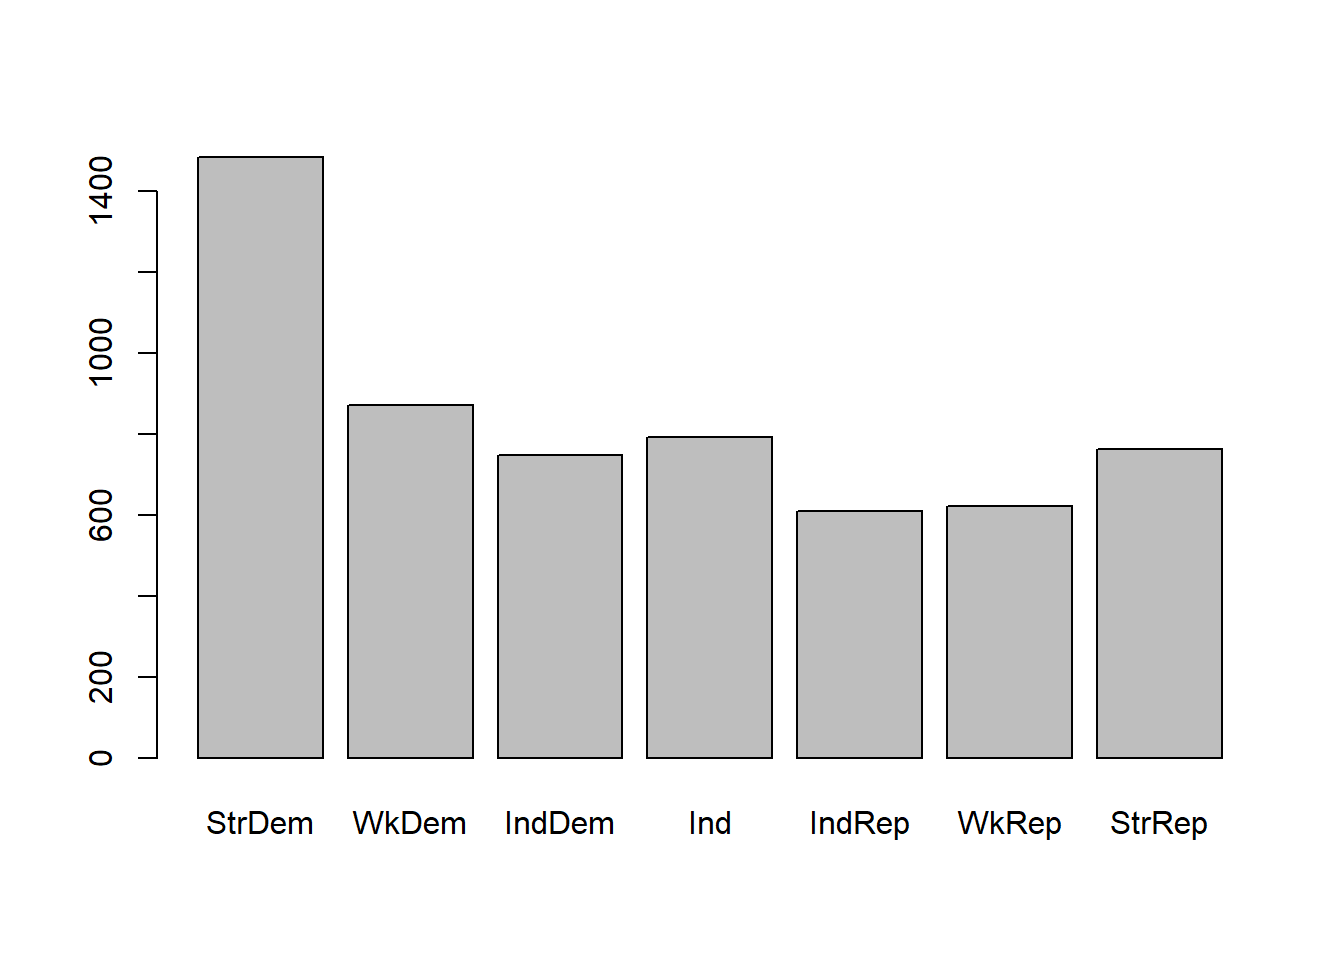
\includegraphics{psc-253-manual_files/figure-latex/unnamed-chunk-12-1.pdf}

\begin{verbatim}
##    Cell Contents 
## |-------------------------|
## |                   Count | 
## |          Column Percent | 
## |-------------------------|
## 
## ============================================
##             pid_3
## envjob_3       Dem      Ind      Rep   Total
## --------------------------------------------
## Envir        1005      721      212    1938 
##             59.82%   38.25%   15.30%        
## --------------------------------------------
## Mid           508      749      525    1782 
##             30.24%   39.73%   37.88%        
## --------------------------------------------
## Jobs          167      415      649    1231 
##              9.94%   22.02%   46.83%        
## --------------------------------------------
## Total        1680     1885     1386    4951 
##             33.93%   38.07%   27.99%        
## ============================================
\end{verbatim}

\subsection{Troubleshooting}\label{troubleshooting-3}

\begin{itemize}
\item
  Make sure that the \texttt{poliscidata} package is loaded. Use
  \texttt{library(poliscidata)} to load.
\item
  The arguments for the independent and dependent variables are just the
  variable names. They do not follow the template of
  \texttt{data\$variable}.
\item
  Crosstabs are used when both the independent and dependent variables
  are categorical. Avoid making a crosstab with numeric data.
\end{itemize}

\bibliography{book.bib,packages.bib}

\end{document}
